\documentclass[conference, a4paper]{IEEEtran}

\usepackage{graphicx}

% used for flow charts
\usepackage{pgf}
\usepackage{tikz}
\usepackage{tikz-qtree}
\usepackage{reotex}

% package url is used when citing a website
\usepackage{url}

\usepackage{amssymb}
\usepackage{amsmath}
\usepackage{cite}
\usepackage[normalem]{ulem}
% for a smile-face character
\usepackage{wasysym}
% listing for codes
\usepackage{listings}
% listing for golang
% NOTE listings-golang.sty is required
\usepackage{listings-golang}
% to support flow graphs
\usepackage{textcomp}
% highlight in tables
\usepackage{xcolor}
\usepackage{colortbl}

\usepackage[linesnumbered, ruled, vlined]{algorithm2e}

% positioning is used for below lef = of
\usetikzlibrary{shapes,shadows,arrows,automata,positioning}
% some tikz-styles on reo channels, not required in papers that have nothing to do with Reo

% finally no todos should exist in this draft
% \usepackage[textsize=tiny]{todonotes}

% -------------------------------------- configurations -----------------------------------------
% declaration of environments
\newtheorem{theorem}{Theorem}
\newtheorem{definition}{Definition}
\newtheorem{example}{Example}

% personal characters
\newcommand{\rblock}[0]{\circleddash}
\newcommand{\rread}[0]{\rhd}
\newcommand{\rnoread}[0]{\oslash}
\newcommand{\smap}[1]{[{#1}]}
\newcommand{\rempty}[0]{\varnothing}

% style of source code environment listings
\lstset{basicstyle=\footnotesize\ttfamily,breaklines=true, frame=shadowbox}
\lstset{numbers=left}
\lstset{xleftmargin=2em, xrightmargin=2em}
\lstset{language=Golang}

% --------------------------------------- information -------------------------------------------
\title{Active Learning from Blackbox to Timed Connectors}
\author{
\IEEEauthorblockN{Yi Li\IEEEauthorrefmark{1}, Yiwu Wang\IEEEauthorrefmark{1} and Meng Sun\IEEEauthorrefmark{1}}
\IEEEauthorblockA{
\IEEEauthorrefmark{1}Department of Informatics, School of Mathematical Sciences, Peking University,
Beijing, China\\
liyi\_math@pku.edu.cn, yiwuwang@126.com, summeng@math.pku.edu.cn
}
}

\begin{document}
\maketitle
\begin{abstract}
  Coordination models and languages play a key role in formally specifying the communication and
  interaction among different components in large-scale distributed and concurrent systems. In this
  paper, we propose an active learning framework to extract timed connector models from black-box
  system implementation. 
  We first introduce parameterized mealy machine as an operational semantic
  model for channel-based coordination language Reo. Parameterized mealy machine serves as a bridge
  between Reo connectors and mealy machines. With the product operator, complex connectors can be
  constructed by joining basic channels and transformed into mealy machines. Moreover, we adapt L*,
  a well-known learning algorithm, to timed connectors (in the form of mealy machines). The new
  algorithm has shown its efficiency in multiple case studies. 
  Implementations of this framework is provided as a package in \texttt{Golang}.
\end{abstract}

\begin{IEEEkeywords}
  Active Learning, Coordination Languages, Timed Connectors
\end{IEEEkeywords}

\section{Introduction}

Distributed real-time embedded system (DRES) is reforming our lives with the name \emph{IoT}, the
internet of things, wherein systems are usually composed of individual components and a
\emph{connector}. Such systems could be distributed logically or physically, which
makes coordination processes even more complicated. In this case, we need to specify these coordination
processes with so-called \emph{coordination languages}, so that formal techniques can be applied to
guarantee their reliability.

\emph{Timed Reo} is a real-time extension of the coordination language \emph{Reo}, by which
coordination process in DRES can be depicted clearly and intuitively. Different formal
semantics are proposed to specify the behavior of timed Reo.
For example, in \cite{DBLP:conf/tase/Meng12}, a UTP-based
(\emph{Unifying Theories of Programming}) semantics is provided to verify connectors as
\emph{designs}. An operational semantics based on \emph{constraint automata} was raised by Baier et
al.\cite{DBLP:conf/sefm/ArbabBBR04}, where a variant of LTL was also proposed to describe the properties of timed connectors.

Formal verification techniques have also been proved applicable in timed connectors, e.g.
\cite{DBLP:conf/tase/LiCWS15} has shown us a comformance testing method on timed connectors.
Bounded model checking methods based on SAT solvers were also adapted in
\cite{DBLP:journals/scp/Kemper12}.
All these solutions seem practical and impressive, however, a common question is faced by
most of them: \emph{how to obtain these formal models?}

\emph{Correctness} of connectors is very much related to some low-level implementation details.
For example, well-writen code may behave dramatically weird with an improper set of concurrency
primitives. Such things happen frequently in embedded systems with different hardware platforms or
operating systems. Consequently, manually modeling an existing connector seems rather unreliable,
even with reference to its source code.

As a branch of \emph{machine learning} technique, active learning offers a way to obtain models from
low-level models. Works in \cite{DBLP:journals/mt/Daelemans10, DBLP:journals/iandc/Angluin87,
DBLP:conf/fase/RaffeltS06} shows interesting examples where active learning is used to extract
\emph{Mealy machines} or \emph{regular languages} without time domain.

\begin{figure}[ht]
  \begin{center}
    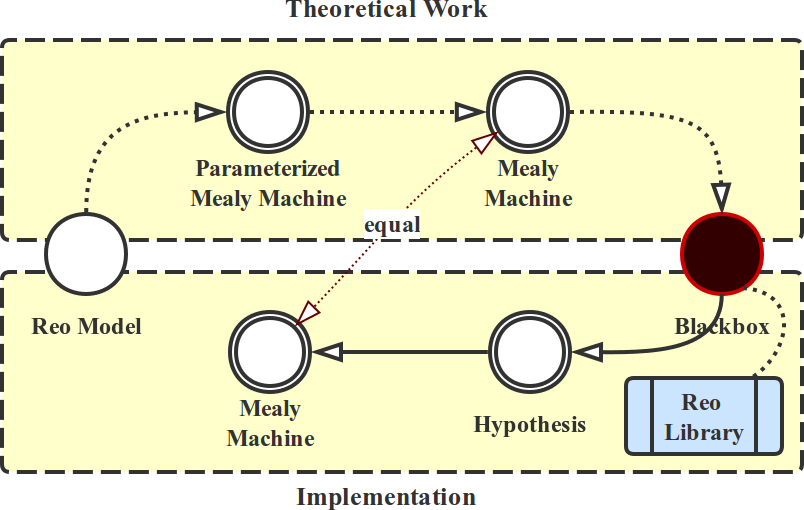
\includegraphics[width=.4\textwidth]{./images/howto.png}
  \end{center}
  \caption{The Active Learning Framework}
  \label{fig:howto}
\end{figure}

To address the problem, we proposed a active learning framework (shown in Figure \ref{fig:howto}) to
automatically extract timed connectors from blackbox models. To achieve this goal, firstly we
present \emph{parameterized Mealy machine} as a parametierized semantics for timed Reo channels,
which is able to generate concrete Mealy machines with a given alphabet. Then the $L*$ algorithm
\cite{DBLP:journals/iandc/Angluin87}
is adapted and optimized to extract Mealy machines with time action from the \emph{connectors in
blackboxes}. 

The rest of the paper is organized as follows. After this general introduction, in Section
\ref{sec:preliminaries} we briefly illustrate some basic concepts, including Reo the coordination
language, Mealy machine, and active automata learning. Section \ref{sec:semantics} defines an
operational semantics of Reo, which is used in Section \ref{sec:activelearning} to show how to
extract Reo models from blackboxes by means of active learning. Finally, in Section
\ref{sec:experiment}, we discuss the implementation and optimization in \texttt{Golang}. 

\section{Preliminaries} 
\label{sec:preliminaries}
\subsection{Reo Coordination Language} 
\label{sec:reo}
We provide here a brief overview of the main concepts in Reo. Further details can be found in
\cite{DBLP:journals/mscs/Arbab04, DBLP:journals/scp/BaierSAR06}.

Reo is a channel based exogenous coordination language proposed by F. Arbab in
\cite{DBLP:journals/mscs/Arbab04}. 
A Reo model, also called \emph{connector}, provides the protocol
that formalizes the communication, synchronization and cooperation among the components which
communicate through the connector. Connectors can be defined without dependence on components,
which makes Reo a powerful ``glue language'' in component-based
development\cite{DBLP:journals/sigsoft/Gill03}.

In Reo, complex connectors are made up of simpler ones. The atomic connectors are called
\emph{channels}, and each of them has two \emph{channel ends}. There are two type of channel ends:
\emph{source} and \emph{sink}. Source channel ends accepts data into the channel, while sink
channels ends dispense them out of the channel. 

\begin{figure}[ht]
  \begin{center}
    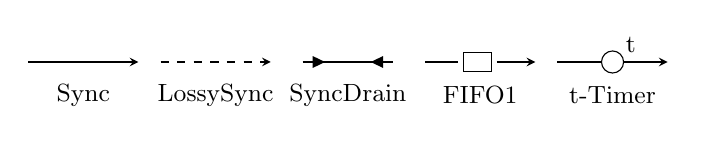
\begin{tikzpicture}[scale=1.4]

\tikzstyle{every node}=[font=\small]
\tikzstyle{label}=[draw=none]

\draw (0.5, -0.3) node[label] {Sync};
\draw (1.7, -0.3) node[label] {LossySync};
\draw (2.9, -0.3) node[label] {SyncDrain};
\draw (4.1, -0.3) node[label] {FIFO1};
\draw (5.3, -0.3) node[label] {t-Timer};

\sync{(0,0)}{(1,0)}{}
\lossysync{(1.2,0)}{(2.2,0)}{}
\syncdrain{(2.4,0)}{(3.4,0)}{}
\fifoe{(3.6,0)}{(4.6,0)}{}

\timer{(4.8,0)}{(5.8,0)}{node [above left] {t}}

\end{tikzpicture}

  \end{center}
  \caption{Basic Reo Channels}
  \label{fig:basic}
\end{figure}

The behavior of some channels are informally described as follows. (Graphical representations
can be found in Figure \ref{fig:basic}).

\begin{itemize}
  \item [-] A \emph{Sync} channel accepts a data item from its source end iff the data item can be
    dispensed to its sink end simultaneously.
  \item [-] A \emph{LossySync} channel is always prepared to accept data items. These items will be
    send to its sink end simutaneously if possible, otherwise they will be dropped.
  \item [-] A \emph{SyncDrain} channel has two source ends and no sink end. It can accept a data
    item through one of its source end iff a data item is also available to accept simultaneously
    through the other end. Then both items will be dropped.
  \item [-] A \emph{FIFO1} channel is an asychronous channel with a buffer cell. It accepts a
    data item whenever the buffer is empty. 
\end{itemize}

Channels are attached on component instances or \emph{nodes}. There are three types of nodes:
\emph{source}, \emph{sink} and \emph{mixed node}, depending on whether all channel ends that
coincide on a node are source ends, sink ends or both. (see in Figure \ref{fig:node})

\begin{figure}[ht]
  \begin{center}
    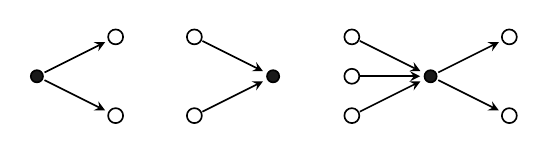
\begin{tikzpicture}[->,>=stealth',shorten >=1pt,auto,node distance=1.6cm,
  semithick]
  \tikzstyle{every node}=[font=\small]

  % source node
  \mixednode{(P-1)}{(-4,0)}{}
  \ionode{(P-2)}{(-3,0.5)}{}
  \ionode{(P-3)}{(-3,-0.5)}{}
  \sync{(P-1)}{(P-2)}{}
  \sync{(P-1)}{(P-3)}{}

  % sink node
  \mixednode{(S-1)}{(-1,0)}{}
  \ionode{(S-2)}{(-2,0.5)}{}
  \ionode{(S-3)}{(-2,-0.5)}{}
  \sync{(S-2)}{(S-1)}{}
  \sync{(S-3)}{(S-1)}{}

  % mixed node
  \ionode{(M-1)}{(0,0.5)}{}
  \ionode{(M-2)}{(0,0)}{}
  \ionode{(M-3)}{(0,-0.5)}{}
  \mixednode{(M-4)}{(1,0)}{}
  \ionode{(M-5)}{(2,0.5)}{}
  \ionode{(M-7)}{(2,-0.5)}{}
  \sync{(M-1)}{(M-4)}{}
  \sync{(M-2)}{(M-4)}{}
  \sync{(M-3)}{(M-4)}{}
  \sync{(M-4)}{(M-5)}{}
  \sync{(M-4)}{(M-7)}{}

\end{tikzpicture}

  \end{center}
  \caption{Source, Sink and Mixed Nodes in Reo}
  \label{fig:node}
\end{figure}



With definition of more basic channels, it's easy to extend Reo to formalize coordination in
different areas. In this paper, we take timed Reo\cite{DBLP:conf/sefm/ArbabBBR04} as our formal
model. Timed Reo includes several timed channels, where the most commonly-used one, called
\emph{timer}, is also shown in Figure \ref{fig:basic}. A t-timer channel accepts any data item from
its source end, and later dispense it to its sink end after a delay of t time units.

Components can be linked to source nodes or sink nodes. A component can write data items to its
corresponding source node only if the data item can be dispensed simultaneously to all source ends
on this node. Similarly, a component can read a data item only if there is at least one readable
sink end on its corresponding node. A mixed node non-determinstically selects and takes a data item
from one of its coincident sink ends and replicates it into all of its coincident source ends.

\begin{figure}[ht]
  \begin{center}
    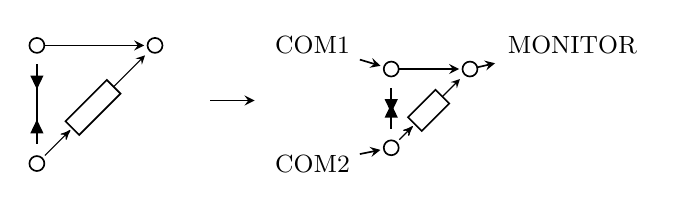
\begin{tikzpicture}[->,>=stealth',shorten >=1pt,auto,node distance=1.6cm,
  semithick]
  \tikzstyle{every node}=[font=\small]

  % draw the alternator
  \ionode{(P-A)}{(0,0)}{}
  \ionode{(P-B)}{(0,-1.5)}{}
  \ionode{(P-C)}{(1.5,0)}{}

  \sync{(P-A)}{(P-C)}{}
  \fifoe{(P-B)}{(P-C)}{}
  \syncdrain{(P-A)}{(P-B)}{}

  % draw the coordination
  \ionode{(C-A)}{(4.5,-0.3)}{}
  \ionode{(C-B)}{(4.5,-1.3)}{}
  \ionode{(C-C)}{(5.5,-0.3)}{}

  \sync{(C-A)}{(C-C)}{}
  \fifoe{(C-B)}{(C-C)}{}
  \syncdrain{(C-A)}{(C-B)}{}

  \node (COM1) at (3.5, 0) {COM1};
  \node (COM2) at (3.5, -1.5) {COM2};
  \node (MONI) at (6.8, 0) {MONITOR};
  \sync{(COM1)}{(C-A)}{}
  \sync{(COM2)}{(C-B)}{}
  \sync{(C-C)}{(MONI)}{}

  \sync{(2.2,-0.7)}{(2.8,-0.7)}{}

\end{tikzpicture}

  \end{center}
  \caption{Coordination with Reo Connectors}
  \label{fig:reoconnector}
\end{figure}

As shown in Figure \ref{fig:reoconnector}, we use a simple example to illustrate how complex
connectors are constructed and used in coordination. In this example, COM1,COM2 and
MONITOR are components. With an \emph{alternator} connector, MONITOR can obtain data items from
COM1 and COM2 alternately. The \emph{alternator} example has been implemented in \texttt{Golang} as
shown in Section \ref{sec:reolib}.
Besides, all the connectors are supposed to be \emph{deterministic} hereinafter to meet the
requirement of active learning algorithm L*.


\subsection{Mealy Machines}

In this work, we use \emph{Mealy machines} to model Reo connectors.
As an extension of \emph{finite state machine}, Mealy machine was first proposed by George. H. Mealy
in \cite{George1955A}. Compared with other variants, Mealy machines are designed to model
reactive systems, where outputs are determined not only by its current state but also the current
inputs. Besides, Mealy machines are supposed to be \emph{input enabled}, which means that all
possible inputs should be acceptable in all states. In other words, if an input is invalid for some
state, we need to manually define an additional state to describe such exceptions.

Various forms of Mealy machines are defined in different works. 
Since active automata learning very much depends on the system-under-learn to be deterministic, in
this paper we formally define a deterministic Mealy machine following
\cite{DBLP:conf/sfm/SteffenHM11}. 

\begin{definition}[Mealy machine]
  A Mealy machine is a 6-tuple $(S, s_0, I, O, \delta, \lambda)$ consisting of the following:
  \begin{itemize}
    \item[-] a finite set of states $S$
    \item[-] a start state (also called initial state) $s_0$ which is an element of $S$
    \item[-] a finite set called the input alphabet $I$
    \item[-] a finite set called the output alphabet $O$
    \item[-] a transition function $\delta : S \times I \rightarrow S$ mapping pairs of a
      state and an input symbol to the corresponding next state.
    \item[-] an output function $\lambda : S \times I \rightarrow O$ mapping pairs
      of a state and an input symbol to the corresponding output symbol.
  \end{itemize}
\end{definition}

We say that a Mealy machine is \emph{finite} if the set $S$ of states and the set $I$ of inputs are
finite. Hereinafter, Mealy machines are always supposed to be finite.

A Mealy machine is in some state $q\in S$ is always ready for inputs at any time. If an input symbol
$i\in I$ is provided, the Mealy machine generates output $o=\lambda(q,i)$ and jumps to state
$q'=\delta(q,i)$. Such an edge is also denoted as $q\xrightarrow[]{i/o}q'$.


\subsection{Active Learning}
In this section, we briefly introduce the main ideas of active automata learning. 

Active learning \cite{settles2010active} is a special case of semi-supervised machine learning where
a learning algorithm is able to interactively query the target systems to obtain the desired outputs
under certain inputs. By well-designed query strategy, active learning is able to obtain more
accurate models with smaller dataset. 

\begin{figure}[ht]
  \begin{center}
    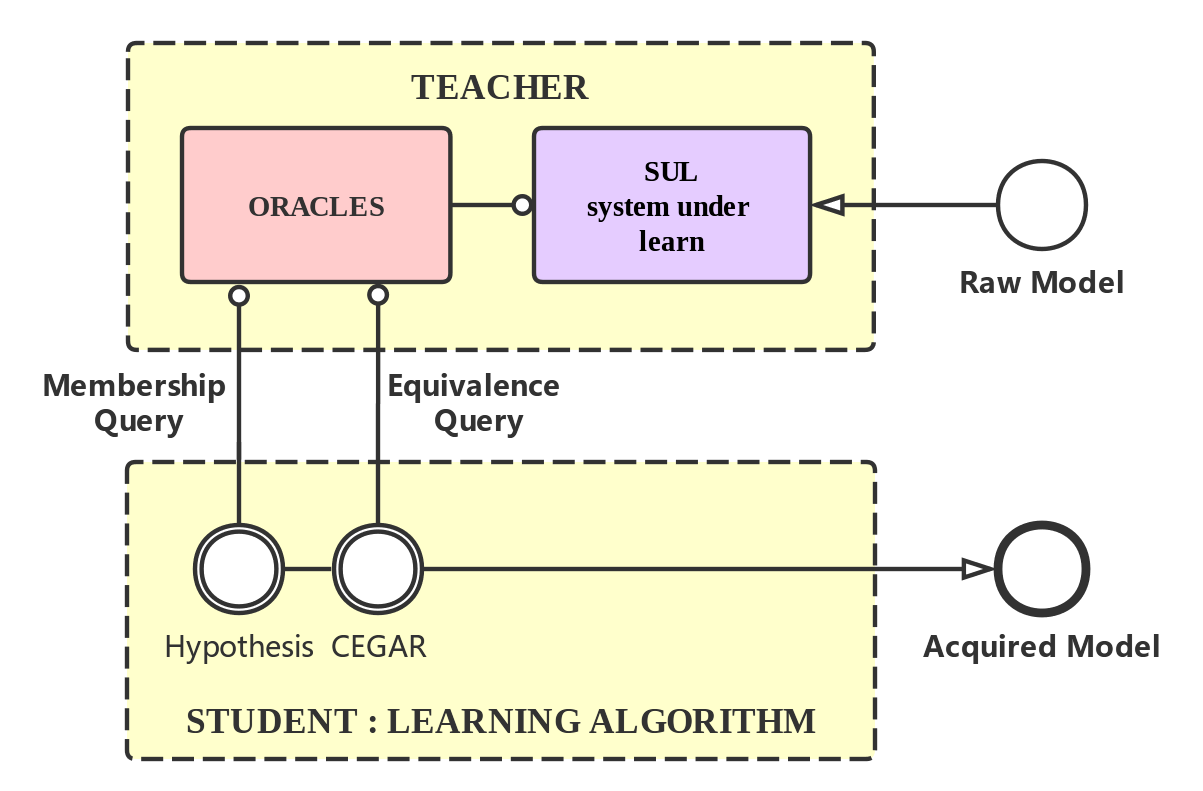
\includegraphics[width=.5\textwidth]{./images/activelearning.png}
  \end{center}
  \caption{Active Automata Learning}
  \label{fig:activelearning}
\end{figure}

Figure \ref{fig:activelearning} shows the sketch of active learning, wherein:
\begin{itemize}
  \item[-] \emph{Teacher} and \emph{Student}: Active learning is an interactive process where
    students ask questions and teachers answer. Here learning algorithm plays the role of student.
  \item[-] \emph{Oracles} is an interface specifying which kind of questions can be answered by the
    teacher.
  \item[-] \emph{SUL} is an abbreviation of System Under Learn. The name comes from a well-known
    concept SUT (System Under Test) in software testing. In this case, we take blackbox models as our
    SULs.
  \item[-] \emph{CEGAR} indicates Counter-Example Guided Abstraction
    Refinement\cite{DBLP:conf/cav/ClarkeGJLV00}. In active learning, we need counter-examples to
    guide us on further quries and cover the undistinguished states.
\end{itemize}

When applying active automata learning on some model, firstly we assume that it should be equivalent
to some \emph{Mealy machine}, in other words, a deterministic model accepting a finite set of input
symbols and mapping them to a finite set of output symbols.

Such a model is encapsulated as a \emph{teacher} by the \emph{Oracle}, which handles
all communication with the model. The oracle also serves as a so-called \emph{Minimal Adequate Teacher}
interface, which is responsible for two types of queries. 

\begin{itemize}
  \item[-] \textbf{Membership Query} (hereinafter referred to as \emph{mq}) The name comes from
    some grammar-learning papers (e.g. \cite{DBLP:journals/iandc/Angluin87}), where \emph{mq} checks
    if a word is a member of certain language defined by the given grammar. When it comes to
    automata learning, \emph{mq} is supposed to provide \emph{simulation results} for given input
    sequences.
  \item[-] \textbf{Equivalence Query} (hereinaftr referred to as \emph{eq}) Given a hypothesis
    (usually constructed by the learning algorithm), \emph{eq} checks whether the hypothesis is
    equivalent to the system-under-learn and generates a counter-example if needed. Generally, 
    \emph{equivalence query} is irrealizable when SUL is a blackbox. So we tactically use membership
    queries to achieve the approximate results.
\end{itemize}

These queries are given by \emph{learning algorithms}, or so-called \emph{students} in Figure
\ref{fig:activelearning}. From the \emph{mq} results, a learning algorithm constructs a
\emph{hypothesis} and then check it with \emph{eq}. If counter-examples are found, we turn back and
repeat the hypothesis construction until the equivalence query returns \emph{true}.

More details on the active automata learning algorithm will be presented in Section
\ref{sec:activelearning}. 

\section{Timed Connectors as Mealy Machines}
\label{sec:semantics}
In this section, we illustrate how to transform a timed connector into a Mealy machine with time
action.
Since time is not involed in original Mealy machine, we first discuss how to formalize the time
dimension in Mealy machine. After that, we present a \emph{parameterized Mealy
machine} as a bridge between connectors and Mealy machines.

\subsection{Time Domain}
Time is involved in several extensions of Reo. For example, timed
Reo\cite{DBLP:conf/sefm/ArbabBBR04}, hybrid Reo\cite{DBLP:conf/icfem/ChenSS14}, etc.
Generally, these models are designed to handle real-time behavior where time is defined in
$\mathbb{R}$. However, we also found some works like \cite{DBLP:journals/fmsd/PrabhakarDM015} where
rational time indeed  makes things easier. In this paper, we choose the rational number field
$\mathbb{Q}$ as our time domain, which simplifies discretization of timed behaviors greatly.

As presented in section \ref{sec:reo}, all real-time behavior in timed Reo comes with the
\emph{t-timer} channels, and the number of these channels are apparently finite. We use
$t_i\in\mathbb{Q}$ to denote the delays of these timer channels, and now we can define a precision
function $prec$.
\[
prec(t_1,\cdots,t_n) = \max_T\{\forall t_i.\exists n_i\in\mathbb{N}.t_i=n_i\cdot T\}
\]
It's easy to prove that such a $T$ is always existing.

In real systems, the concept \emph{time precision} is well known with other names like ``clock-period''.
Most of the time, we know the clock-period of some hardware components, even without any idea of its
structure. With such precision $dt$ given, it's reasonable to assume that all $t$-timers are actually
$ndt$-timers. In following sections, we'll use $n$-Timers instead.

Besides, we're going to add a ``T'' action in Mealy machines. It indicates that a transition
will take a time unit to finish.

\subsection{Parameterized Mealy Machine}
We present a model named \emph{parameterized Mealy machine} (hereinafter referred to as PMM)
to model timed connectors. PMM is supposed to behave as a middle representation between Mealy
machines and timed connectors. Connectors are firstly defined as parameterized Mealy machines, and
composed by production operator and link operator. Then, concrete Mealy-machine model can be
generated from the PMM model.
Following the formal definition of Mealy machine in Section \ref{sec:preliminaries}, we define the
\emph{parameterized Mealy machine} as follows. 

\begin{definition}[Parameterized Mealy Machine]
  A \emph{Parameterized Mealy Machine} is defined as a 6-tuple $\mathcal{PM}=\langle
  S, s_0, I, O, \delta, \lambda\rangle$ with a parameter named $\Sigma$ where 
  \begin{itemize}
    \item[-] $\Sigma$, the parameter, is a \emph{finite} datum alphabet
    \item[-] $S$ is a function that maps an alphabet to a \emph{finite} set of
      states. We use $S(\Sigma)$ to denote the state set.
    \item[-] $I$ is a finite set of source-ends.
    \item[-] $O$ is a finite set of sink-ends.
    \item[-] $s_0$ is the initial state. It satisfies $\forall \Sigma,s_0\in S(\Sigma)$
    \item[-] $\delta$ maps a \emph{finite} datum alphabet to an \emph{output function}. We use
      $\delta(\Sigma):S(\Sigma)\times Input(\Sigma,I,O)\rightarrow Output(\Sigma,I,O)$ to denote the
      output function.
    \item[-] $\lambda$ maps an alphabet to a \emph{transition function}. We use
      $\lambda(\Sigma):S(\Sigma)\times Input(\Sigma,I,O)\rightarrow S(\Sigma)$ to denote the transiton
      function.
  \end{itemize}
\end{definition}

In the definition above, \emph{Input} and \emph{Output} are used to generate input actions
and output actions from the corresponding alphabets and source/sink ends. The value of $Input(\Sigma,I,O)$ is
defined as a set of functions on $I\cup O$ where $\forall f\in Input(\Sigma,I,O)$ and an additional
\emph{time action} T, we have
\[
\forall i\in I\backslash\{T\}, f(i)\in \Sigma\cup\{\bot\}\land \forall o\in
O,f(o)\in\{\rread, \rnoread\}
\]
where we use $\rread$ to indicate that an end-sink is ready for write, and $\rnoread$ otherwise. Note
that a $\bot$ means that there is \emph{no} data items on a source (or sink) end. In the same way,
$Output(\Sigma,I,O)$ is defined as a set of functions on domain $O$, with an additional symbol
$\rblock$ indicating an input failure. Similarly, $\forall f\in Output(\Sigma,I,O), f\neq \rblock$
implies
\[
\forall o\in O, f(o)\in \Sigma\cup\{\bot\}
\]

\begin{example}[Input and Output]
  If we have a simple alphabet with only one item $d_0$, a source-end named $A$, and a
  sink-end named $B$, the input actions would be
  \begin{small}
    \begin{eqnarray*}
      Input(\{d_0\},\{A\},\{B\}) &=& \{\{A:d_0,B:\rread\},\{A:d_0,B:\rnoread\}, \\
      & & \{A:\bot,B:\rread\},\{A:\bot,B:\rnoread\},T\}
    \end{eqnarray*}
  \end{small}
  and its output actions
  \[
  Output(\{d_0\},\{A\},\{B\}) =\{\{B:d_0\},\{B:\bot\}, \rblock\}
  \]
\end{example}

If there is no data item written to any sink ends, we use $\varnothing$ to denote such an empty
output. For example, in the case given above, $\{B:\bot\}$ can be briefly rewritten as $\varnothing$.

Parameterized Mealy machines can be seen as an abstract form of Mealy machines, which means that we
still need a convert function between the two models.

\begin{definition}[Concretize Mapping]
  We use $\smap{\mathcal{PM}}_{\Sigma}$ to denote the concrete Mealy machine which is determined by
  an abstract parameterized Mealy machine $\mathcal{PM}$ and the alphabet $\Sigma$. Apparently
  $\smap{\mathcal{PM}}_{\Sigma}$ can be described as
  \begin{eqnarray*}
    \smap{\mathcal{PM}}_{\Sigma} &=& 
    \langle
    \mathcal{PM}.S(\Sigma), \mathcal{PM}.s_0, \\
    & & Input(\Sigma, \mathcal{PM}.I), Output(\Sigma, \mathcal{PM}.O), \\
    & & \mathcal{PM}.\delta(\Sigma), \mathcal{PM}.\lambda(\Sigma),
    \rangle
  \end{eqnarray*}
\end{definition}

Now we can use parameterized Mealy Machines to define a new semantics for timed Reo. Here we
take one asynchronous channel (FIFO1), one asynchronous channel (Sync) and one timed channel (Timer)
as examples.

\begin{example}[PMM Semantics of FIFO1 channel]
  \label{example:pmmfifo}
  The semantics of FIFO channel with source end $A$ and sink end $B$ can be defined as follows.
  \begin{itemize}
    \item[-] $S(\Sigma)=\{q_0\}\cup\{q_d|d\in\Sigma\}$
    \item[-] $I=\{A\}$, $O=\{B\}$, $s_0=q_0$
    \item[-] output function
      \begin{displaymath}
        \delta(\Sigma)(s,i)=\left\{
        \begin{array}[ht]{ll}
          (B:\bot) & s=q_0\land i=(A:\_,B:\rnoread) \\
          (B:\bot) & s=q_d\land i=(A:\_,B:\rnoread) \\     
          (B:d) & s=q_0\land i=(A:d,B:\rread)\\
          (B:d) & s=q_d\land i=(A:\_,B:\rread)\\
          \rblock & s=q_d\land i=(A:d,B:\rnoread) \\
          \rblock & s=q_0\land i=(A:\bot,B:\rread) \\
        \end{array}
        \right.
      \end{displaymath}
    \item[-] transition function
      \begin{displaymath}
        \lambda(\Sigma)(s,i)=\left\{
        \begin{array}[ht]{ll}
          q_d & s=q_0\land i=(A:d,B:\rnoread) \\
          q_d & s=q_{d'}\land i=(A:d,B:\rread) \\
          q_0 & otherwise \\
        \end{array}
        \right.
      \end{displaymath}
  \end{itemize}
\end{example}

Besides, the concrete Mealy machine (where $\Sigma=\{a\}$) is shown in Figure \ref{fig:pmmfifo},
where labels of edges are in form of $\frac{input}{output}$.
\begin{figure}[ht]
  \begin{center}
    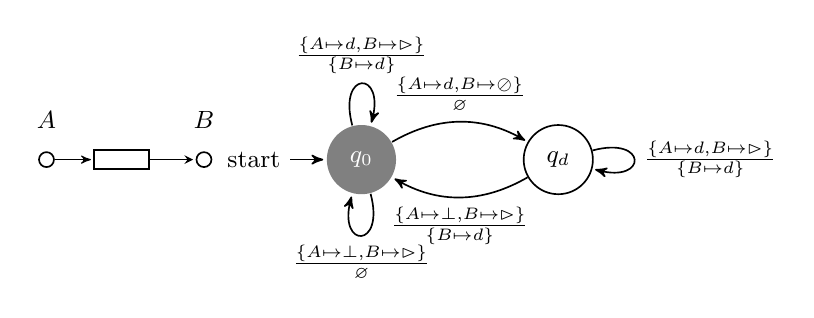
\begin{tikzpicture}[->,>=stealth',shorten >=1pt,auto,node distance=1.6cm,
  semithick]
  \tikzstyle{every node}=[font=\small]
  \ionode{(P-A)}{(-4,0)}{(-4,0.5) node {$A$}}
  \ionode{(P-B)}{(-2,0)}{(-2, 0.5) node {$B$}}
  
  \fifoe{(P-A)}{(P-B)}{}

  \tikzstyle{every state}=[fill=white,text=black,font=\small]
  \tikzstyle{init}=[fill=gray,draw=none,text=white]

  \node[initial,state,init] (Q0)                     {$q_{0}$};
  \node[state]         (QA)  [right = of Q0]    {$q_{d}$};

  \path
  (Q0)
  edge  [bend left]     node {$\frac{\{A\mapsto d, B\mapsto \rnoread\}}{\varnothing}$} (QA)
  edge  [loop below]    node {$\frac{\{A\mapsto \bot, B\mapsto \rread\}}{\varnothing}$} (QA)
  edge  [loop above]    node {$\frac{\{A\mapsto d, B\mapsto \rread\}}{\{B\mapsto d\}}$} (QA)
  (QA)
  edge  [bend left]     node {$\frac{\{A\mapsto \bot,B\mapsto \rread\}}{\{B\mapsto d\}}$} (Q0)
  edge  [loop right]    node {$\frac{\{A\mapsto d,B\mapsto \rread\}}{\{B\mapsto d\}}$} (QA)
  ;
\end{tikzpicture}


  \end{center}
  \caption{PMM-based Semantics of $\smap{FIFO1}_\Sigma$, where $\Sigma=\{a\}$}
  \label{fig:pmmfifo}
\end{figure}

\begin{example}[PMM Semantics of Sync channel]
  The PMM-based semantics of a Sync channel with a source-end A and a sink-end B can be defined as:
  \begin{itemize}
    \item[-] $S(\Sigma)=\{q_0\}$, $I=\{A\}$, $O=\{B\}$, $s_0=q_0$
    \item[-] output function
      \begin{displaymath}
        \delta(\Sigma)(s,i)=\left\{
        \begin{array}[ht]{ll}
          (B:\bot) & s=q_0\land i=(A:\bot,B:\rnoread) \\
          (B:d) & s=q_0\land i=(A:d,B:\rread)\\
          \rblock & s=q_0\land i=(A:\bot,B:\rread) \\
          \rblock & s=q_0\land i=(A:d,B:\rnoread) \\
        \end{array}
        \right.
      \end{displaymath}
    \item[-] transition function $\lambda(\Sigma)(s,i)=q_0$.
  \end{itemize}
\end{example}

\begin{example}[PMM Semantics of n-Timer channel]
  Considering an n-Timer channel with a source-end A and a sink-end B, we define its PMM-based
  semantics as:
  \begin{itemize}
    \item[-] $S(\Sigma)=\{q_{i,d}|0\leq i\leq n, d\in \Sigma\}\cup\{q_0\}$
    \item[-] $I=\{A\}$, $O=\{B\}$, $s_0=q_0$
    \item[-] output function
      \begin{displaymath}
        \delta(\Sigma)(s,i)=\left\{
        \begin{array}[ht]{ll}
          (B:d) & s=q_{n,d}\land i=(A:d,B:\rread)\\
          \rblock & s=q_{n,d}\:\land \\
          & (i=T\lor i=(A:\_,B:\rnoread) \\
          \rblock & s=q_{j,d}\land 1 \leq j < n\land \\
          & (i=(A:\_,B:\rread)\lor \\
          & i=(A:d,B:\_))\\
          (B:\bot) & otherwise\\
        \end{array}
        \right.
      \end{displaymath}
    \item[-] transition function
      \begin{displaymath}
        \lambda(\Sigma)(s,i)=\left\{
        \begin{array}[ht]{ll}
          q_{j+1,d} & s=q_{j,d}\land i=T\land0 < j < n\\
          q_0 & s=q_{n,d}\land i=(A:\bot,B:\rread) \\
          q_{0,d} & s=q_{n,d'}\land i=(A:d,B:\rread) \\
          q_{0,d} & s=q_0 \land i=(A:d,B:\_) \\
          s & otherwise \\
        \end{array}
        \right.
      \end{displaymath}
  \end{itemize}
\end{example}

Similarly, we can use parameterized mealy machines to define the semantics of other basic timed Reo
channels. Now we're going to show how to compose these channels into complicated connectors.

\begin{definition}[Production Operator]
  Now we're going to define the production operator \emph{prod} of two parameterized Mealy machines as,
  \[
  prod(PM_1,PM_2)=PM_3
  \]
  as follows. Here we assume that $PM_2.O\cap PM_1.I=\varnothing$
  \begin{itemize}
  	\item[-] $\forall\Sigma, PM_3.S(\Sigma)=PM_1.S(\Sigma)\times PM_2.S(\Sigma)$
    \item[-] $PM_3.I=PM_1.I\cup PM_2.I-PM_1.O$
    \item[-] $PM_3.O=PM_1.O\cup PM_2.O-PM_2.I$
  \end{itemize}
  \emph{(Here we assume that sink ends of $PM_1$ can be connected to source ends $PM_2$, but not
  vise versa)}
  \begin{itemize}
    \item[-] $PM_3.s_0=(PM_1.s_0, PM_2.s_0)$
    \item[-] $\forall\Sigma, PM_3.\delta(\Sigma)((s_1,s_2), i)=$
      \begin{displaymath}
        \left\{
        \begin{array}[ht]{ll}
          (Out_1 + Out_2)\downarrow_{PM_3.O} & Out_1\neq\rblock\land Out_2\neq\rblock \\
          \rempty & i = T \\
          \rblock & otherwise \\
        \end{array}
        \right.
      \end{displaymath}
      where we have
      \begin{itemize}
        \item[*] $In_1 = i\downarrow_{PM_1.I}$
        \item[*] $Out_1 = PM_1.\delta(\Sigma)(s_1,In_1)$
        \item[*] $In_2 = (Out_1 + i)\downarrow_{PM_2.I}$
        \item[*] $Out_2 = PM_2.\delta(\Sigma)(s_2,In_2)$
      \end{itemize}
    \item[-] $\forall\Sigma, PM_3. \lambda(\Sigma)((s_1,s_2),i)=(s_1',s_2')$
      where we have
      \begin{itemize}
        \item[*] $s_1' = PM_1.\lambda(\Sigma)(s_1,In_1)$
        \item[*] $s_2' = PM_2.\lambda(\Sigma)(s_2,In_2)$
      \end{itemize}
  \end{itemize}
\end{definition}

The idea in \emph{production} is quite simple. The output of $PM_1$ would be provided as part of the
input of $PM_2$. Time actions T is only executed simutaneously between $PM_1$ and $PM_2$.

As mentioned in the notation above, we cannot connect a sink end of $PM_2$ to a source end of
$PM_1$, which makes it difficult to construct connectors like alternator in Figure
\ref{fig:reoconnector}. To address the problem, we define a \emph{link} operation to connect sink
ends and source ends in the same connector.

\begin{definition}[Link Operator]
  The \emph{link} operation constructs connector by connecting a sink end $OUT$ to a source end $IN$
  within the same connector.   
  \[
  PM' = link(PM, OUT, IN)
  \]
  Here we asuume that $IN\in PM.I$ and $OUT\in PM.O$.

  \begin{itemize}
  	\item[-] $\forall\Sigma, PM'.S(\Sigma)=PM.S(\Sigma)$
    \item[-] $PM'.I=PM.I-\{IN\}$
    \item[-] $PM'.O=PM.O-\{OUT\}$
    \item[-] $PM'.s=PM.s$
    \item[-] $\forall\Sigma, i\in Input(\Sigma,PM'.I,PM'.O)$, $PM'.\delta(\Sigma)(s, i)=$
      \begin{equation}
        \label{equ:existd}
        PM.\delta(\Sigma)(s,T)\downarrow_{PM'.O}
      \end{equation}
      if $i=T$. When $i$ is a non-time action, we need to check whether there's a data item
      $d\in\Sigma$
      satisfies
      \[
      PM.\delta(\Sigma)(s,i\cup\{IN:d\})\downarrow_{OUT} = d
      \]
      if the formula is satisfied, we have $PM'.\delta(\Sigma)(s, i)=$
      \[
      PM.\delta(\Sigma)(s,i\cup\{IN:d\})\downarrow_{PM'.O}
      \]
      otherwise $PM'.\delta(\Sigma)(s, i)=\rblock$
    \item[-] $\forall\Sigma, i\in Input(\Sigma,PM'.I,PM'.O).'$ the transition
      function can be defined as $PM.\lambda(\Sigma)(s,i)=$
      \begin{displaymath}
        \left\{
        \begin{array}[ht]{ll}
          PM.\lambda(\Sigma,T) & i=T \\
          PM.\lambda(\Sigma,i\cup\{IN:d\}) & \exists d\in\Sigma \mbox{ satisfes Equation
          \ref{equ:existd}} \\
          s & otherwise \\
        \end{array}
        \right.
      \end{displaymath}
  \end{itemize}
\end{definition}

With \emph{link} and \emph{prop} defined, complex connectors can be formed by simple channels in
form of \emph{parameterized Mealy machines}. It will be transformed into a concrete Mealy machine
later once the alphabet $\Sigma$ is provided.

\section{From Blackbox to Timed Connectors} 
\label{sec:activelearning}
In this section, we show how to use L* algorithm to extract models from blackboxes in  3 steps:
\emph{constructing hypothesis}, \emph{enclosing hypothesis} and \emph{checking hypothesis}. Besides,
we assume that input symbols and output symbols of the blackbox have been provided as $\mathcal{I}$
and $\mathcal{O}$.

\subsection{Observation Table}
As mentioned above, membership queries provide us information with the form $mq(s)=o$, where $s$ is
an input sequence in $\Sigma^{+}$. Now the question is, \emph{how to find the connection between
such query results and Mealy machines?}

Generally, Mealy machines are composed of \emph{states} and \emph{transitions}.
Provided with a Mealy machine $m$, any input sequence in $m.I^+$ leads to a unique state. 
Such a sequence is called an \emph{access sequence} of this state.
Particularly, we use $\varepsilon$, the \emph{empty sequnce}, to denote the initial state.
Similarly, if a blackbox model has the same bahavior with a Mealy machine, we can use access
sequences to label its states and, in the same way, input actions to label its transitions.
For example, we consider a Mealy machine which is staying in some state labelled by $s$. With an
action $a$ provided, the Mealy machine will jump to a new state labelled by $s'=sa$ and generate an
output $mq(sa)$. 

Different access sequences may lead to similar states. For example, a 2-Timer channel will dispense
any accepted data item in 2 time units. After that, the state of this channel is exactly same as its
initial state. Here \emph{suffixes} are used to distinguish different states as shown in the
following definition, where $D$ is initialized as $\mathcal{I}$. Under such a suffix set, two states
are considered different only when they have different one-step behaviors.

\begin{definition}[Equivalence under Suffixes]
  provided with two access sequences $s_1,s_2$ and a set of suffixes $D\subset\mathcal{I}^+$, we say
  the corresponding states of $s_1$ and $s_2$ are equivalent under $D$ (denoted as $s_1\sim_D s_2$)
  iff $\forall d\in D, mq(s_1d) = mq(s_2d)$.
\end{definition}

Since all this \emph{inputs} and \emph{outputs} can be observed outside the
model, we can use the same notations to describe a black box as a hypothetical Mealy machine.
Following this idea, \emph{Observation Tables}, proposed in \cite{DBLP:journals/iandc/Angluin87},
shows a tabular form of such hypothetical models. In observation tables, rows represent states with
label of their access sequences and columns are labelled with suffixes. Successors of a state $s$ is,
intuitively, denoted as extended access sequences $sa$ where $a$ is a single input action. 
A cell with column-label $d$ and row-label $s$ should contain the value $mq(sd)$. Algorithm
\ref{alg:buildtable} shows how to build such an observation table.

\begin{algorithm} 
  \caption{BuildTable} 
  \label{alg:buildtable}
  \KwIn{Oracle interface $mq$, Input actions $\mathcal{I}$, suffix set $D$}
  \KwOut{Observation table $obs$} 
  $obs$ initialized as empty\;
  $unclosed=\{\varepsilon\}$\;
  \Repeat{$unclosed=\varnothing$}
  {
    $next=\{st|\forall s\in unclosed,\forall t\in \mathcal{I}\}$\;
    append $unclosed$ to $obs$\;
    $unclosed=\{seq\in next|\forall a\in obs, seq \not\sim_D a\}$\;
  }
  \Return $obs$\; 
\end{algorithm}

Taking a 2-Timer channel as an example, we now illustrate how this algorithm works. 
We assume that the source end of this 2-Timer channel is $A$, the sink end is $B$ and the alphabet
is $\{a\}$. We briefly denote $\{A:a,B:\rnoread\}$ and other input/output actions in form of
$a,\rnoread$.

Firstly, $obs$ is initialized as empty and the empty sequence $\varepsilon$ is pushed in $unclosed$.
Then we will explore all the access sequences in $unclosed$ and calculate its successors. Here the
$unclosed$ set consists of access sequences that has no equivalent fellow with less length. 
For example, figure \ref{fig:hypo} shows the $obs$ of a 2-Timer channel after the first
iteration. The five successors of $\varepsilon$ is presented as the bottom part of the table, where
four are equivalent with $\varepsilon$ but $a,\rnoread$ is not. Therefore, we take $a,\rnoread$ as a
brand-new state and all of its successors need further exploration (see in the hypothesis Mealy
machine presented in the following figure).

\begin{figure}[ht]
  \begin{center}
    \begin{displaymath}
      \begin{array}{l||ccccc}
        \hline
        & a,\rread & \bot,\rread & a,\rnoread & \bot,\rnoread & T\\
        \hline\hline
        \varepsilon & \rblock & \rblock & \rempty & \rempty & \rempty \\
        \hline
        a,\rread & \rblock & \rblock & \rempty & \rempty & \rempty \\
        \bot,\rread & \rblock & \rblock & \rempty & \rempty & \rempty \\
        \rowcolor[gray]{.9}
        a,\rnoread & \rblock & \rblock & \rblock & \rempty & \rempty \\
        \bot,\rnoread & \rblock & \rblock & \rempty & \rempty & \rempty  \\
        T & \rblock & \rblock & \rempty & \rempty & \rempty \\
        \hline
      \end{array}
    \end{displaymath}
    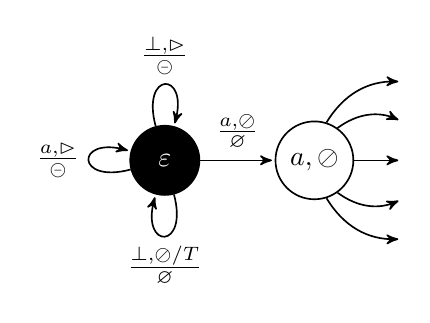
\begin{tikzpicture}[->,>=stealth',shorten >=1pt,auto,node distance=1.9cm,
  semithick]
  \tikzstyle{initial}=[fill=black, text=white]

  \node[initial,state] (Q0)               {$\varepsilon$};
  \node[state]         (Q1) [right of=Q0] {$a,\rnoread$};
  
  \path
  (Q0) edge [loop left]  node {$\frac{a,\rread}{\rblock}$} (Q0)
  (Q0) edge [loop above] node {$\frac{\bot,\rread}{\rblock}$} (Q0)
  (Q0) edge              node {$\frac{a,\rnoread}{\rempty}$} (Q1)
  (Q0) edge [loop below] node {$\frac{\bot,\rnoread/T}{\rempty}$} (Q0)
  (Q1) edge [bend left]  node {} (3,1)
  (Q1) edge [bend left]  node {} (3,0.5)
  (Q1) edge              node {} (3,0)
  (Q1) edge [bend right] node {} (3,-0.5)
  (Q1) edge [bend right] node {} (3,-1)
  ;
\end{tikzpicture}


  \end{center}
  \caption{Observation Table and Corresponding Hypothesis}
  \label{fig:hypo}
\end{figure}

In the second iteration, we explore the successors of $a,\rnoread$. Fortunately we find that every
successor has a shorted equivalence fellow (\emph{itself}). Consequently, the algorithm terminates
with a closed hypothesis where all the unclosed edge shown in Figure \ref{fig:hypo} turn into
self-loop.

\begin{figure}[ht]
  \begin{center}
    \begin{displaymath}
      \begin{array}{l||ccccc}
        \hline
        & a,\rread & \bot,\rread & a,\rnoread & \bot,\rnoread & T\\
        \hline\hline
        \varepsilon & \rblock & \rblock & \rempty & \rempty & \rempty \\
        \hline
        a,\rread & \rblock & \rblock & \rempty & \rempty & \rempty \\
        \bot,\rread & \rblock & \rblock & \rempty & \rempty & \rempty \\
        a,\rnoread & \rblock & \rblock & \rblock & \rempty & \rempty \\
        \bot,\rnoread & \rblock & \rblock & \rempty & \rempty & \rempty  \\
        T & \rblock & \rblock & \rempty & \rempty & \rempty \\
        \hline
        a,\rnoread-a,\rread & \rblock & \rblock & \rblock & \rempty & \rempty \\
        a,\rnoread-\bot,\rread & \rblock & \rblock & \rblock & \rempty & \rempty \\
        a,\rnoread-a,\rnoread & \rblock & \rblock & \rblock & \rempty & \rempty \\
        a,\rnoread-\bot,\rnoread & \rblock & \rblock & \rblock & \rempty & \rempty \\
        a,\rnoread-T & \rblock & \rblock & \rblock & \rempty & \rempty \\
        \hline
      \end{array}
    \end{displaymath}
  \end{center}
  \caption{A Closed Observation Table}
  \label{fig:hypo2}
\end{figure}

\subsection{Counter-Examples' Analysis} 
Apparently, the closed hypothesis presented in Figure \ref{fig:hypo2} is not equal to the 2-Timer
channel. It's easy to find a counter-example $s=a,\rnoread-T-T-\bot,\rread$ where $mq(s)=a$ while
according to the hypothesis, the result shoud have been $\rempty$. In this section, we show how to
find and analyze counter-examples, which is mainly based on \cite{DBLP:conf/sfm/SteffenHM11}. 

Firstly, we give a formal definition of \emph{counter-examples}. With a observation table $obs$ and
a sequence $s$, we use $acc(s)$ to denote the access sequence of $obs\xrightarrow{s}$ and $hq(s)$ to
denote the corresponding output.

\begin{definition}[Counter-Example]
  We use $hq$ to denote execution result of the hypothetical Mealy machine, sequence $s$ is called a
  counter-example iff $mq(s)\neq hq(s)$.
\end{definition}

Now we consider the reason that lead to existance of counter examples. Since
the suffix set $D$ is used to distinguish different states, the existance of counter-examples
shows that the current suffix set $D$ is not powerful enough to distinguish all different states.

Considering a counter example $s$, we have
\[
\mbox{MaxSuffix}(s)=\max_d\{s=s'd, mq(acc(s')d)\neq mq(s)\}
\]
Since $mq(acc(s))=hq(s)\neq mq(s)$ and $mq(s) = mq(s)$, the existance of such $d$ is easy to prove.
After appending $d$ in $D$, we explain the closedness will be violated.

The whole L* algorithm can be concluded as follows.
\begin{algorithm} 
  \caption{L*} 
  \label{alg:lstar}
  \KwIn{Oracle interface $mq,eq$, Input actions $\mathcal{I}$}
  \KwOut{Observation table $obs$} 
  $D=I$\;
  \Repeat{$ce=true$}{
    $obs$ = BuildTable($mq$, $\mathcal{I}$, $D$)\;
    $ce=eq(obs)$\;
    \If {$ce!=true$} {
      D.append(MaxSuffix(s))\;
    }
  }
  \Return $obs$\; 
\end{algorithm}




\section{Experiments} 
\label{sec:experiment}

Both \emph{Reo Coordination Models} and \emph{Adapted L* Algorithm} are implemented in
Golang\cite{golang}.

Golang (or Google Go) is a rising programming language started by Google Inc. The language is widely
known for its elegant design and impressive efficiency. Moreover, the concurrency model of Golang
comes from CSP\cite{DBLP:books/ph/Hoare85}. As a channel-based model, CSP shares a similar idea with
Reo and makes our implementation much more natural.

All the following experiments are coded under Golang \emph{1.2.1} and executed on a laptop with 8GB
of RAM and a Core i7-3630 CPU. The source code is available at
\url{https://github.com/liyi-david/reo-learn}.

\subsection{Case Study}
A simple example of timed connector is presented to show how L* works.
\begin{figure}[ht]
  \begin{center}
    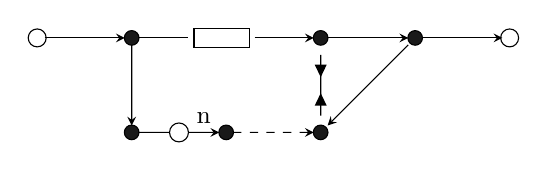
\begin{tikzpicture}[scale=1.2]
  \tikzset{every node} = [font=\small]

  \ionode{(P-A)}{(0,0)}{}
  \ionode{(P-B)}{(5,0)}{}
  \mixednode{(P-C)}{(1,0)}{}
  \mixednode{(P-D)}{(3,0)}{}
  \mixednode{(P-E)}{(4,0)}{}
  \mixednode{(P-F)}{(1,-1)}{}
  \mixednode{(P-G)}{(2,-1)}{}
  \mixednode{(P-H)}{(3,-1)}{}

  \fifoe{(P-C)}{(P-D)}{}
  \syncdrain{(P-D)}{(P-H)}{}
  \sync{(P-A)}{(P-C)}{}
  \sync{(P-C)}{(P-F)}{}
  \sync{(P-D)}{(P-E)}{}
  \sync{(P-E)}{(P-B)}{}
  \sync{(P-E)}{(P-H)}{}
  \lossysync{(P-G)}{(P-H)}{}

  \timer{(P-F)}{(P-G)}{node [above] {n}}

\end{tikzpicture}

  \end{center}
  \caption{Expiring FIFO1 Channel (ExpFIFO1)}
  \label{fig:expfifo}
\end{figure}

Informally speaking, an expiring FIFO1 channel with \emph{timeout} $n$ is able to accept a data item
and stored it in the buffer cell for $n$ time units. If a read operation on $B$ is performed within
$n$ time units, it will obtain the data item successfully and clear the buffer. However, the data
item would be dropped if no read operation comes.

\begin{figure}[ht]
  \begin{center}
    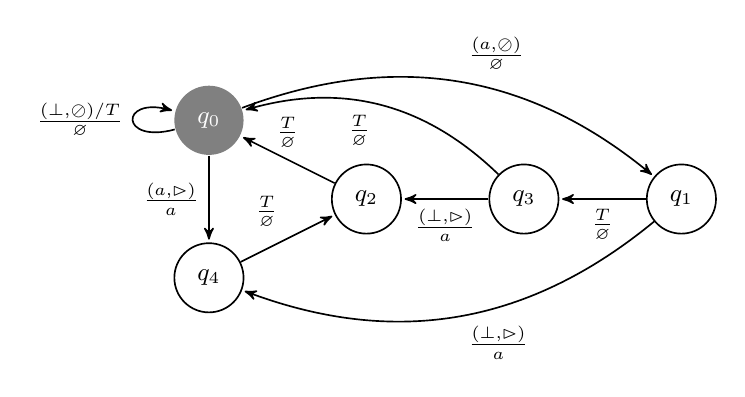
\begin{tikzpicture}[->,>=stealth',shorten >=1pt,auto,node distance=1.9cm,
  semithick]
  \tikzstyle{initial}=[fill=gray,text=white]
  \tikzstyle{every node}=[font=\small]
  \tikzstyle{nodraw}=[draw=none]

  \node[initial,state, nodraw] (Q0) at (0,1)   {$q_0$};
  \node[state]         (Q1) at (6,0)   {$q_1$};
  \node[state]         (Q2) at (2,0)  {$q_2$};
  \node[state]         (Q3) at (4,0)   {$q_3$};
  \node[state]         (Q4) at (0,-1)  {$q_4$};
  
  \path
  (Q0) edge [bend left]  node         {$\frac{(a,\rnoread)}{\rempty}$} (Q1)
  (Q0) edge              node [left]  {$\frac{(a,\rread)}{a}$} (Q4)
  (Q0) edge [loop left]  node         {$\frac{(\bot,\rnoread)/T}{\rempty}$} (Q0)
  (Q1) edge              node         {$\frac{T}{\rempty}$} (Q3)
  (Q1) edge [bend left]  node         {$\frac{(\bot,\rread)}{a}$} (Q4)
  (Q2) edge              node [above] {$\frac{T}{\rempty}$} (Q0)
  (Q3) edge              node         {$\frac{(\bot,\rread)}{a}$} (Q2)
  (Q3) edge [bend right] node         {$\frac{T}{\rempty}$} (Q0)
  (Q4) edge              node         {$\frac{T}{\rempty}$} (Q2)
  ;
\end{tikzpicture}


  \end{center}
  \caption{Learn Result of The ExpFIFO1 where $n=2,\Sigma=\{a\}$}
  \label{fig:expfifosemantics}
\end{figure}

Figure \ref{fig:expfifosemantics} shows the learning result of this example.
To simplify the graph, we ignore the all the trivial transitions $\frac{\bot,\rnoread}{\rempty}$
and block transitions. More details of this case can be found in our \emph{github repo}.

\subsection{Performance Optimization}
As a well-known learning algorithm, L* has proved its efficiency in models without time.
However, when dealing with timed connectors, the algorithm failed to meet our expectation.

\begin{table}[ht]
  \renewcommand{\arraystretch}{1.3}
  \caption{Time-Cost Analysis}
  \label{tabel:timecost}
  \centering
  \begin{tabular}{l||rrr}
    \hline
    & FIFO & Alternator & Gate \\
    \hline\hline
    Membership Query(s) & 41.571 & 126.468 & 169.161 \\
    Hypothesis Query(s) & 0.001 & 0.003 & 0.004 \\
    Total Time(s) & 41.715 & 165.114 & 247.098 \\
    Membership Query(\%) & 99.6 & 76.6 & 68.5 \\
    \hline
  \end{tabular}
\end{table}

As shown in Table \ref{tabel:timecost}, time consumption mainly comes from membership queries.
Since time is involved in our model, it's inevitably that simulation takes time to behave normally.
Even worse, since our models are treated as blackbox. With no access to inner behaviour of the
connectors, it's almost impossible to accelerate the simulation process.

Fortunately, there are still other optimization solutions. After reviewing our algorithm, we found
that simulations on similar sequences were invoked frequently:

\begin{itemize}
  \item When constructing \emph{Obs} tables, there are lots of redundant calls to membership
    queries. For example, a sequence with prefix 'aa' and suffix 'b' is exactly same as another one
    with prefix 'a' and suffix 'ab'.
  \item Simulation on mealy machines can provide multi-step output. Consequently, if we have
    simulated an 'abc' sequence, there's no reason to perform simulation on an 'ab' sequence.
\end{itemize}

If previous simulation results are stored in a well-maintained cache, the time-cost in
simulation process could be reduced signficiantly. In this work, we use a multiway tree to buffer
these results.

\begin{table}[ht]
  \renewcommand{\arraystretch}{1.3}
  \caption{Reduction of Membership Queries}
  \label{tabel:cacheoptimization}
  \centering
  \begin{tabular}{l||rrr}
    \hline
    & FIFO & Alternator & Gate \\
    \hline\hline
    Original Algorithm & 93 & 880 & 1034 \\
    Cached Algorithm & 90 & 725 & 707 \\
    Reduction Rate & 3.2\% & 21.4\% & 31.6\% \\
    \hline
  \end{tabular}
\end{table}

With cache applied, we have made considerable reduction on the calls of membership queries. The results
can be found in Table \ref{tabel:cacheoptimization}.

\subsection{An Example of the Reo Package }
\label{sec:reolib}

Our implementation in \texttt{Golang} is well-prepared not only for academic use
but also for practical concurrent programming. The following code shows how to compose an alternator
connector (see in Figure \ref{fig:reoconnector}) in \texttt{Golang}. An intact version of this example
can be found in our github repo.

\begin{lstlisting}
func alternator(A, B, C Port) {
  M := MakePorts(6)

  // definition of channels
  go ReplicatorChannel(A, M[0], M[1])
  go ReplicatorChannel(B, M[2], M[3])
  go MergerChannel(M[4], M[5], C)

  go SyncdrainChannel(M[1], M[2])
  go SyncChannel(M[0], M[4])
  go FifoChannel(M[3], M[5])
}
\end{lstlisting}

Provided with the source and sink nodes, \emph{alternator} function creates a series of basic
channels and mixed nodes (named \emph{Port}) to serve as the alternator connector we need. Now we
can activate the components and using \emph{alternator} function to coordinate them.

\begin{lstlisting}
A,B,C := MakePorts(3)
alternator(A, B, C)

go sender(A, "MSG A")
go sender(B, "MSG B")
go monitor(C)
\end{lstlisting}

In this case, \emph{sender} are goroutines (basic parallel units in \texttt{Golang}) that keep
sending certain messages to some given port (A and B). A \emph{monitor} keep trying to read data
items from the sink end C and print them on the screen. Finally, we have an interleaved sequence of
``MSG\_A'' and ``MSG\_B''.
 
\section{Conclusion and Future Work}
In this paper, we come up with an approach to learn timed connectors from blackboxes. We define
the \emph{parameterized Mealy machine} to serve as an operational semantics of Reo. Then we
describe a set of basic channels with parameterized Mealy machine, which can be used to construct
complex connectors by means of the production operator and link operator.
Besides, we show that every connector can be transformed into a Mealy
machine with time action T, and such Mealy machines can be extracted by an improved version of
well-knwon active learning algorithm L*.

The original L* algorithm run into the bottleneck when time is involved. By a tree-style cache, we
make significant reduction on membership queries and, in turn, improve the performance of learning
algorithm. As a by-product, we also encapsulate the Reo connector as a distributable package which
could contribute to concurrent programming.

Our future works would mainly focus on better support of dense time. To describe dense
time behavior, the Mealy machine model needs a lot of changes instead of a simple T action. Besides,
we will also try to improve our algorithm to handle non-deterministic behaviors. This is not a brand
new topic \cite{DBLP:journals/eceasst/VolpatoT15}, but we believe that there is still room for
improvement.  
\bibliographystyle{abbrv}
\bibliography{bib}

\end{document}
